\subsection{Organizzazione del codice}
La suddivisione del codice rispecchia fortemente il design architetturale generale descritto in precedenza.
\begin{center}
    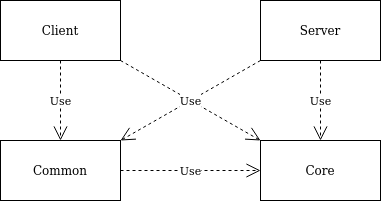
\includegraphics[scale=0.5]{moduli}
\end{center}
Sono stati realizzati 4 moduli:
\begin{itemize}
    \item Core: comprende tutte le entità necessarie alla realizzazione del gioco e le regole per poter portare avanti una partita, è l’unico tra i moduli totalmente indipendente dagli altri.
    \item Common: codice comune alle parti di client e server, per la maggior parte definisce i messaggi utilizzati per lo scambio di informazioni
    \item Client: contenente tutto ciò che concerne il client, interfaccia utente, parte di comunicazione con il server e di aggiornamento dello stato della partita
    \item Server: contenente tutta la parte di gestione delle lobby e delle partite in corso
\end{itemize}

\subsection{Core}
Il core modella al suo interno tutte le entità del gioco Machiavelli reale, come le carte, il mazzo e il tavolo da gioco, come anche la GameInterface, cioè un insieme di funzioni che gli altri moduli del progetto devono usare per poter interagire con le entità.
Tali funzioni infatti modellano tutte le azioni che un giocatore può svolgere nel gioco reale.
\newline
E’ importante sottolineare il fatto che sia immutabile e quindi non conserva alcuno stato interno.
Esso deve essere utilizzato all’esterno sfruttando appunto le API messe a disposizione.

\subsubsection{Entità}
\begin{center}
    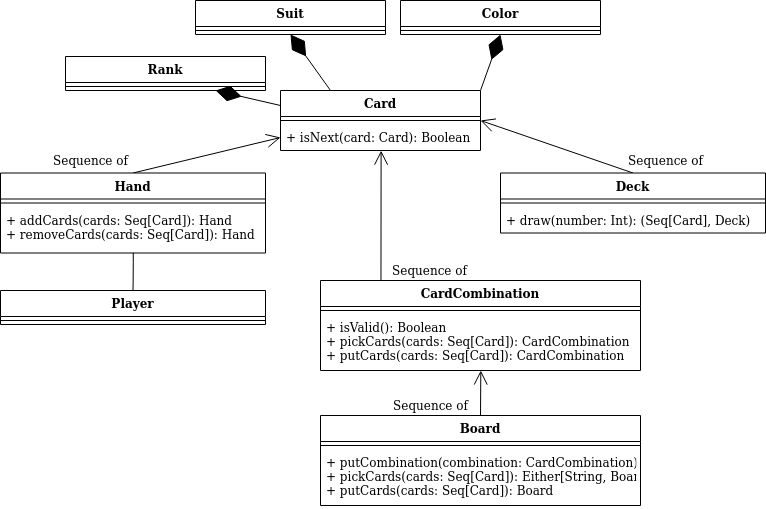
\includegraphics[width=\textwidth]{classi-Page-1}
\end{center}
Le entità di gioco sono elencabili come:
\begin{itemize}
    \item Card, corredata da un Rank (valore nominale), un Seme e un Colore.
    E’ stato modellato anche il caso del Rank Asso come 14-esimo possibile valore, per poterne effettuare la validazione qualora si trovasse dopo il Re (13-esimo valore) in una combinazione
    \item Player, composta da un username, un id e una mano
    \item Hand, che contiene i metodi per poter aggiungere (o rimuovere) carte dal tavolo alla mano (dalla mano al tavolo) e per ordinare le carte
    \item CardCombination, rappresenta un tris, poker o una scala ordinata
    \item Deck, rappresenta il mazzo
    \item Board, rappresenta il tavolo di gioco e contiene un insieme di CardCombination e i relativi metodi per poterle aggiungere, rimuovere e aggiornare
\end{itemize}

\subsubsection{Prolog}
Per la gestione delle regole di validazione, sii è deciso di utilizzare questo linguaggio in quanto è possibile esprimerle in maniera totalmente dichiarativa conciso ed efficiente.
La libreria utilizzata è TuProlog.
\begin{center}
    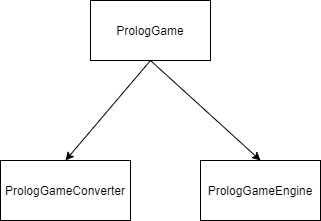
\includegraphics{prolog}
\end{center}
Di seguito vengono descritte le classi:
\begin{itemize}
    \item il PrologGame espone tutte le funzionalità implementate attraverso tale linguaggio.
    Ogni qualvolta che si deve eseguire una funzionalità in Prolog, è necessario richiamare un metodo di questa classe corrispondente all’azione di Prolog.
    In particolare permette di creare le carte corredate da un valore, un seme e un colore per formare il deck di gioco, di eseguire la validazione di una sequenza di carte, che sia essa una scala, tris o poker e ne esegue l’ordinamento per seme e per valore.

    \item il PrologEngine esegue effettivamente le azioni di Prolog.
    Si è deciso di realizzare un piccolo DSL che permettesse di facilitare l’utilizzo della libreria TuProlog e di aumentarne l’espressività del codice.
    Dopo aver caricato la specifica teoria, il PrologEngine esegue le funzioni in grado di:
    \begin{itemize}
        \item risolvere un singolo obiettivo o più obiettivi
        \item verificare se un obiettivo ha successo
        \item se vi sono altre soluzioni dopo averne trovata almeno una
        \item estrarre i valori dalle variabili, dopo l’esecuzione di un predicato, tramite il metodo bindingVars
    \end{itemize}

    \item il PrologGameConverter espone le funzioni in grado di formulare obiettivi nel giusto ‘formato’ in Prolog e di convertire il risultato ottenuto dal PrologEngine nel tipo corretto, a seconda dell’utilizzo.
    In particolare, grazie all’utilizzo dell’oggetto PrologUtils, espone metodi in grado di ‘pulire’ (da caratteri non conformi) il risultato del Prolog dopo averlo convertito in stringa.
    Questo è stato reso necessario poiché quando si dava in input un obiettivo che conteneva una lista di tuple (ogni carta è una tupla che contiene nel seguente ordine valore, seme e colore), il risultato risultava essere ‘sporco’ da caratteri estranei rispetto al predicato dato in input.
    Di fatto l’oggetto PrologUtils espone delle funzioni e una Regex che lavorano su stringhe e sostituiscono i caratteri non accettati.
    La classe converter permette infine di gestire la validazione di specifici casi, ad esempio una combinazione contenente uno o più assi.
    Questo perché l’asso in una combinazione che forma una scala, può essere posto prima del due o dopo del re e quindi a fini di validazione, per la teoria definita, l’asso può assumere sia il valore 1, sia il 14.
    Il metodo OptionalValueAce gestisce i casi appena descritti cambiandone il valore in modo conforme.

\end{itemize}

\subsubsection{Game Interface}
\begin{center}
    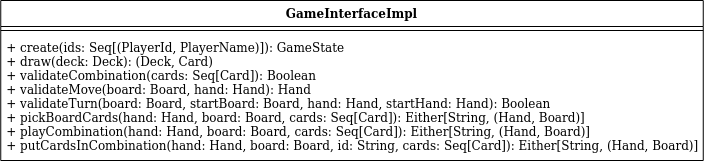
\includegraphics[width=\textwidth]{classi-Page-2.png} %todo: add diagram.
\end{center}

\subsection{Client}
%todo: Add Client class diagram.

\subsubsection{MVC}
Per la parte client dell’applicazione si è scelto di utilizzare una architettura basata sul pattern MVC\@.
Questa ci ha consentito di tenere, anche all’interno del client, un buon livello di separazione tra le singole classi.
\newline
All’avvio dell’applicazione AppLauncher avvia MainController, che istanzia una istanza di View che fa da contenitore per entrambe le due parti di gioco (quella di avvio e quella di partita).
MainController avvierà prima StartupController per la parte di iscrizione alle lobby, e una volta ricevuto da quest’ultimo l'evento di creazione della partita, avvia il GameController.
Ciascun controller setta nella view il proprio Stage e istanzia la classe Service, che nel MVC gioca il ruolo di model.
%todo: Add another diagram.
Come si può notare dallo schema, il controller, per notificare eventi alla view, avendo creato il relativo Stage, richiama i metodi che questo espone.
\newline
Allo stesso tempo, in creazione passa anche onViewEvent(), una funzione che viene invocata dalla view ogni qualvolta debba notificare un evento al controller.
Questa funzione prende in input un oggetto di tipo case class/object che estende la sealed class ViewEvent.
Questa scelta di utilizzare da una parte l’interfaccia e dall’altra un metodo a callback è dovuta al fatto che logicamente, la view può notificare al controller qualsiasi tipo di evento, e sarà il controller a decidere quale di questi gestire;
al contrario la view espone solamente le funzionalità che espone nella propria interfaccia.
\newline
Simile è anche l’interazione tra Service e Controller.
Il Controller avendo creato il Service ha il suo riferimento ed invoca i metodi che questo espone nella sua interfaccia.
Allo stesso tempo passa in creazione il metodo notifyEvent() che viene chiamato dal Service quando deve notificare un cambiamento di stato.

\subsubsection{View}
In ciascuno Stage vengono caricate le varie scene, ciascuna delle quali ha un interfaccia di metodi che possono essere chiamati dallo Stage che la contiene.
\newline
Per velocizzare la creazione degli elementi di view più utilizzati, sono state creati degli object che contengono i factory methods per creare i relativi elementi:
\begin{itemize}
    \item ScalavelliButton, factory per gli oggetti Button
    \item ScalavelliLabel, factory per gli oggetti Label
    \item ScalavelliAlert, factory per gli oggetti Alert
    \item ScalavelliTextField, factory per gli oggetti Button
\end{itemize}
L’object CardUtils è invece una utility che permette di ottenere il path dell’immagine della carta da gioco a partire dall’entità Card.
Si è scelto di gestire la visualizzazione degli alert e degli errori direttamente da Stage in quanto deve essere indipendente dalla scena in cui ci si trova.
Tutti i metodi che agiscono sugli elementi già renderizzati dalla view e gli aggiornamenti di stato hanno l’esigenza di agire sullo stesso thread di ScalaFX. Per poter ottenere questo risultato sono stati eseguiti all’interno della chiamata a Platform.runLater().

\subsubsection{Lobby}

\paragraph{Controller}
StartupController avvia la view che permette all’utente di selezionare la modalità con cui partecipare ad una lobby e l’inserimento dei suoi dati.
Una volta fatto questo, tramite l’interazione con StartupService comunica al server la scelta dell’utente e attende una risposta.

\paragraph{View}
%todo: Add Lobby View diagram.
La parte di view si caratterizza di 4 scene che vengono caricate all’interno di StartupStage.
La scena principale permette di scegliere tra le 3 modalità di iscrizione a disposizione:
\begin{itemize}
    \item Iscrizione ad una lobby pubblica, in base al numero di players selezionati.
    \item Iscrizione ad una lobby privata, inserendo un codice segreto.
    \item Creazione di una lobby privata, selezionando il numero di membri necessari per questa lobby.
\end{itemize}
Alla selezione di una di queste modalità, viene caricata una nuova scena, alla quale viene passato un listener di tipo StartUpSceneListener che tramite callback permette di reagire alle azione di submit() e della pressione del tasto back.
\newline
Ciascuna scena scena eredita da StartupBaseScene e si compone di 3 parti:
\begin{itemize}
    \item StartupSceneTopBar, che contiene il pulsante per tornare alla schermata precedente
    \item StartupSceneBottomBar, che contiene il pulsante di invio e la rotella di caricamento mentre si è in attesa della creazione di una partita.
    \item Un nodo centrale in cui è possibile l’inserimento dei dati o, nel caso della creazione di un codice segreto, la visualizzazione di quest’ultimo.
\end{itemize}

\subsubsection{Model}
La parte di model del client è rappresentata dai trait StartupService e GameService con tutte le strutture a loro collegate.
Rappresentano il punto in cui risiede tutta la business logic del client.
Sono entrambi delle interfacce che espongono tutte le funzionalità rese disponibili dall’applicazione, su cui in controller si appoggiano per eseguire tutte le operazioni risultanti dalle azioni utente effettuate attraverso l’interazione con la view.
Permettono quindi di astrarre ai componenti utilizzatori le modalità con cui le varie azioni vengono risolte, ad esempio decidere se risolverle in locale o in remote contattando il server.
È solamente in questa parte del codice client che sono presenti riferimenti al framework akka.
A differenza del server, il client non è stato modellato totalmente ad attori, che sono stati invece utilizzati solo per la parte di comunicazione con il server tramite scambio di messaggi.

\paragraph{StartupService}
%todo: Add StartupService Diagram
È il componente che si occupa della gestione della lobby.
La sua funzione primaria, essendo la lobby gestita totalmente lato server, è quella di comunicare con quest’ultimo.
La connessione al server viene fatta tramite tramite il metodo actorSelection messo a disposizione dall’unica istanza dell’oggetto ActorSystem presente nell’object ActorSystemManager, in caso di connessione avvenuta, si ottiene il riferimento all’attore remoto serverLobbyRef responsabile per la gestione delle lobby, che viene utilizzato per l’invio dei successivi messaggi di richiesta di aggiunta alla lobby.
I messaggi di risposta del server vengono invece ricevuti tramite l’attore StartupActor, creato all’inizializzazione dell’oggetto sempre tramite l’istanza di ActorSystem, il cui riferimento viene passato al server al momento della connessione.
Questo attore ha l’unica funzione di ricevere i messaggi inviati dal server e di redirezionarli tramite il trait StartupServerResponsesListener che richiede in costruzione.
La decisione di comunicare con il server su due vie separate è stata fatta per evitare duplicazione di messaggi: far fare tutto a StartupActor avrebbe richiesto l’invio di messaggi a quest’ultimo che a sua volta avrebbe dovuto inviarli al server.
Il risultati delle varie operazioni vengono poi notificati al controller attraverso la funzione notifyEvent richiesta in costruzione, a cui viene passato un oggetto di tipo GameStartupEvent.
Il risultato della fase di lobby è l’oggetto GameMatchInformations, che racchiude tutte le informazioni necessarie a poter avviare la partita lato client, come l'id del giocatore e la reference all'attore remoto del server.

\paragraph{GameService}
È il componente che si occupa di gestire lato client tutta la fase di gioco.
Come il componente descritto in precedenza per la fase di lobby, anche questo consiste in un’interfaccia che espone tutti i metodi corrispondenti alle funzionalità rese disponibili dal client di gioco.
La sua implementazione GameServiceImpl è poi caratterizzata da diversi elementi, ciascuno dei quali gestisce una componente specifica del gioco.
Il riferimento all’attore server remoto serverActorRef utilizzato per inviare messaggi al server
ClientGameActorRef, il riferimento all’attore locale responsabile di ricevere i messaggi inviati dal server, con una struttura analoga a quella descritta precedentemente per la lobby.
GameStateStore utilizzato per mantenere lo stato locale della partita ed aggiornarlo a seguito delle azioni compiute dall’utente o dagli aggiornamenti ricevuti dal server.
History, una struttura dati immutabile utilizzata per salvare lo storico degli stati risultanti dalle mosse eseguite dall’utente durante il turno.
In seguito ad ogni mossa effettuate dal giocatore durante il turno viene aggiornata e utilizzata poi per ripristinare lo stato a delle versioni precedenti a seguito delle azioni di undo/redo.
GameInterface, l’interfaccia core utilizzata per eseguire in locale le azioni di gioco effettuate durante il turno.
In costruzione riceve poi una funzione che utilizza per notificare al chiamante (in questo caso il controller) gli aggiornamenti di stato e gli altri eventi di sistema.
%todo: Add GameService Diagram
Il grafico di cui sopra mostra la sequenza di operazioni che avvengono durante il turno di un giocatore quando quest’ultimo esegue una mossa:
\begin{itemize}
    \item Un chiamante invoca un metodo del GameService corrispondente a un’azione di gioco
    \item GameService risolve l’azione per mezzo di gameInterface
    \item Sulla base dell’output della funzione invocata su gameInterface viene aggiornato lo stato locale di gioco tramite un metodo di gameStateStore
    \item Il nuovo stato di gioco viene salvato sulla history
    \item Il nuovo stato di gioco viene notificato al componente sottostante per mezzo della funzione notifyEvent ottenuta in costruzione
\end{itemize}
Nel caso di una mossa eseguita in remoto la chiamata al gameInterface è sostituita con un messaggio inviato al server, mentre manca l’aggiornamento della history che viene utilizzata solamente durante la gestione locale del turno.

\subsection{Server}
È la componente che permette lo svolgersi del gioco in modalità multiplayer del gioco, ogni sessione utente è possibile distinguerla in 2 fasi principali:
\begin{itemize}
    \item una fase di startup o lobby: in questa fase l’utente, una volta avviata l’applicazione, cerca di connettersi al server inviandogli i dati necessari per poter trovare una partita.
    Il server dalla sua rimane costantemente in attesa di connessioni di client.
    Una volta connessi e ottenute le loro informazioni di gioco li inserisce all’interno della lobby, in attesa che si verifichino le condizioni necessari affinché una partita possa essere generata.
    Al raggiungimenti di tali condizioni, viene creata una partita, inserendo i giocatori che vengono rimossi dalla lobby.
    \item una fase di gioco: questa fase gestisce lo svolgersi della partita ed è ulteriormente suddivisa in 2 sotto fasi
    \begin{itemize}
        \item Fase di inizializzazione, in cui i client ricevono un messaggio del fatto che la partita è stata trovata e ne danno conferma al server.
        Il server aspetta i messaggi da tutti i client e una volta ricevuti, viene generato lo stato iniziale della partite e comunicato ai giocatori, dopo di che il gioco può iniziare.
        \item Fase di gioco, in cui il server si occupa di far proseguire il gioco, determinando il giocatore corrente, ricevendo le sue mosse, aggiornando lo stato in maniera ciclica, fino al verificarsi delle condizioni di terminazione del gioco.
        Il client si occupa di intercettare tutti le azioni effettuate dall’utente durante la partita, di comunicarle al server al termine del turno e di ricevere le varie informazioni sullo stato di avanzamento della partita.
    \end{itemize}
\end{itemize}

\subsubsection{Lobby}
\begin{center}
    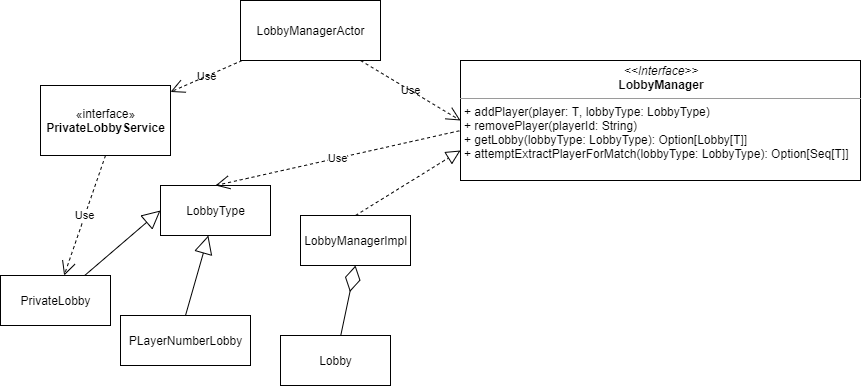
\includegraphics[width=\textwidth]{server-classi-lobby}
\end{center}
LobbyManagerActor è l’attore che si occupa di tutta la parte di gestione della fase di startup del gioco, è stato implementato estendendo il trait Actor di akka, rendendo quindi possibile la ricezioni di messaggi provenienti dai giocatori client.
Parte della logica di questo componente è stata poi portata fuori in altre strutture dati cercando di seguire il principio di Separation of Concerns.
Lobby è la struttura base che rappresenta una lista di giocatori accomunati dalle stesse preferenze riguardanti il numero di giocatori necessari per poter iniziare una partita.
LobbyManager è invece il componente che si occupa di mantenere i riferimenti a tutte le lobby create fino a quel momento, espone i metodi per inserire, rimuovere o estrarre i giocatori da una specifica lobby.
Per fare ciò mantiene una Lobby in corrispondenza di ogni LobbyType, che rappresenta l’informazione sulle caratteristiche di una lobby.

\paragraph{Modellazione delle lobby private}
La lobby privata presenta la caratteristica di una normale lobby di avere associato un valore corrispondente al numero di giocatori tale da poter essere estratti per formare un partita, oltre a questo ha un codice univoco per poterla identificare univocamente tra le tante.
PrivateLobbyService supporta la creazione private, generando un id univoco ogni volta che ne viene richiesta una nuova.

\paragraph{Interazione con il client}
\begin{center}
    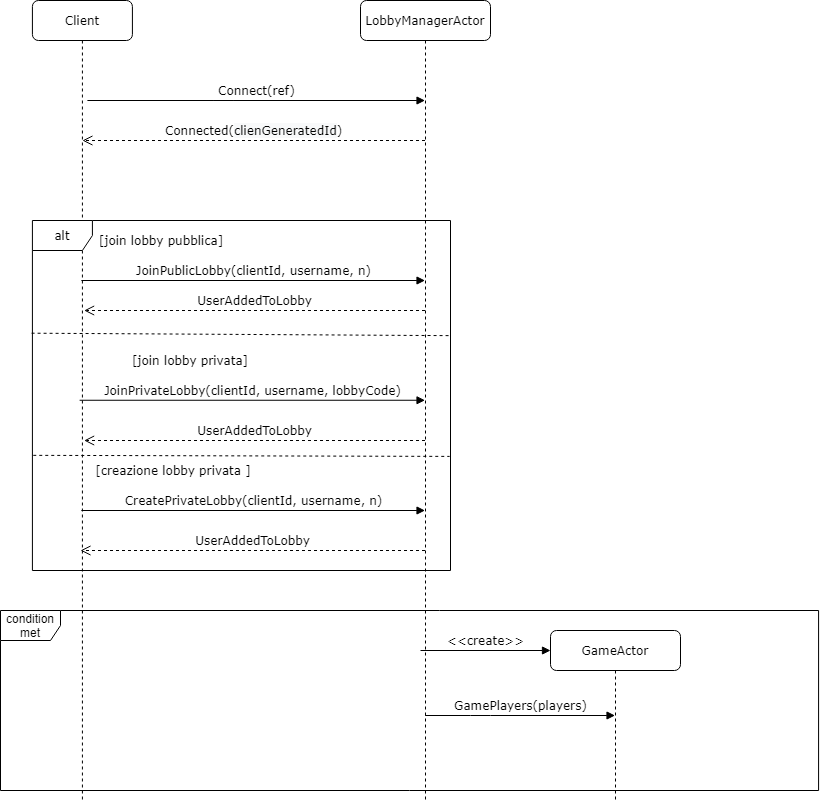
\includegraphics[width=\textwidth]{server-diagramma-attivita-lobby}
\end{center}
La sequenza di operazioni necessaria poter entrare in lobby e partecipa ad una partita è la seguente:
\begin{itemize}
    \item un client invia un messaggio Connect al server passandogli il riferimento all’attore client a cui quest’ultimo dovrà rispondere, a seguito del quale viene generato un id univoco che viene restituito al client
    \item il client dopo aver scelto le preferenze di gioco, richiede al server di essere aggiunto ad una lobby (privata o pubblica) o di crearne una sua privata.
    Il server aggiunge il client alla lobby corrispondente rispondendo al client con un messaggio di avvenuta aggiunta.
    \item dopo aver aggiunto un giocatore ad una lobby, il server controlla se sono verificate le condizione per l’avvio di una nuova partita sulla lobby corrente tramite il metodo di LobbyManager attemptExtractPlayerForMatch che tenta di estrarre la lista di giocatori.
    In caso positivo i giocatori vengono rimossi dal sistema di lobby, viene creato un attore specifico per la partita GameMatchManagerActor a cui vengono passate i loro riferimenti e che da quel momento in poi si occuperà di tutta la fase di gioco.
\end{itemize}

\subsubsection{Game}
\begin{center}
    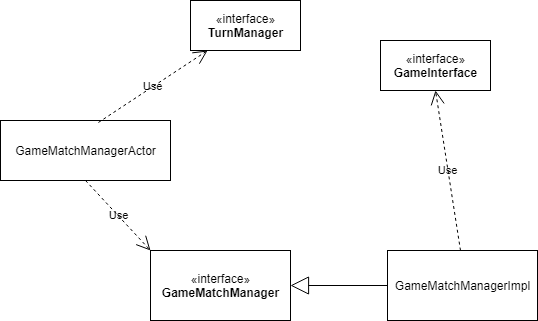
\includegraphics{server-game-classes}
\end{center}
\textit{GameMatchManagerActor} è l’attore server che occupa della gestione di una partita, creato dall’attore Lobby descritto in precedenza.
Fa uso di due interfacce principali:
\begin{itemize}
    \item \textit{TurnManager} è la struttura che gestisce la rotazione dei turni dei giocatori, possiede la lista dei giocatore e la logica per determinare quello successivo a partire da quello corrente.
    \item \textit{GameMatchManager}, la cui implementazione è l’unica classe server che ha riferimento al core, espone i metodi necessari a creare lo stato iniziale della partita e a determinare lo stato successivo della partita sulla base dell’azione compiuta dal giocatore a fine turno.
\end{itemize}
Mantiene inoltre lo stato globale della partita, ad ogni suo aggiornamento lo trasmette a tutti giocatori connessi.
Per questioni di sicurezza, ad ogni giocatore non viene inviato lo stato globale ma uno stato parziale ricavato da esso con il metodo broadcastGameStateToPlayers, contenente le sole informazioni di interesse al giocatore (ad esempio l’informazione sul deck rimane solo al server, come anche la composizione delle mani degli avversari, che il giocatore corrente ovviamente non deve conoscere).

\paragraph{Comunicazione nella fase di inizializzazione della partita}
\begin{center}
    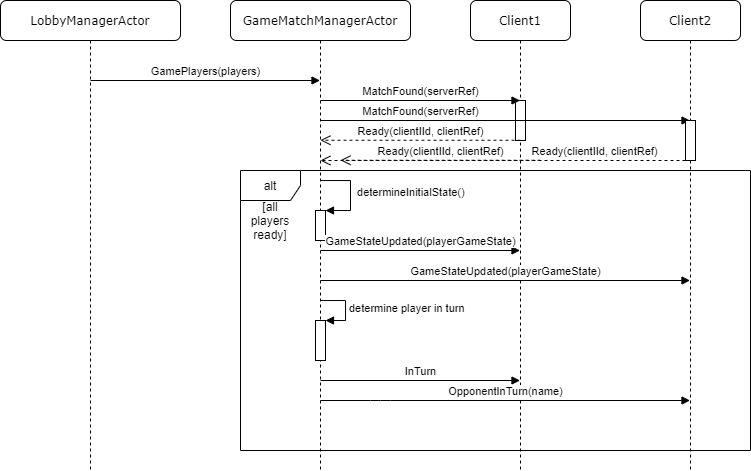
\includegraphics[width=\textwidth]{server-sequence-diagram-inizializzazione-gioco}
\end{center}
Una volta creato dall’attore lobby:
\begin{itemize}
    \item rimane in attesa di un messaggio di inizializzazione (GamePlayers) da parte di quest’ultimo, contenente le informazioni dei giocatori.
    \item Notifica poi i giocatori che la partita è stata trovata tramite il messaggio MatchFound
    \item rimane in attesa del loro messaggio di conferma Ready, contenente oltre all’id del giocatore il riferimento all’attore a cui inviare i successivi messaggi.
    \item Ricevuti tutti i messaggi di conferma la partita viene inizializzata, viene generato lo stato iniziale ed inviato ai vari giocatori, determinato e notificato il giocatore in turno.
\end{itemize}

\paragraph{Comunicazione durante il turno di gioco}
\begin{center}
    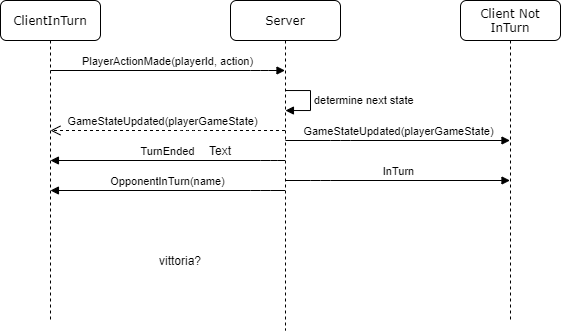
\includegraphics[width=\textwidth]{server-sequence-diagram-turno}
\end{center}
Una volta inizializzato il gioco e stabilito il giocatore corrente, il server rimane in attesa dell’azione di fino turno (le restanti azioni effettuate durante il turno sono gestite in locale come descritto in precedenza).
Dopodiché determina lo stato successivo sulla base dell’azione effettuata che può essere:
\begin{itemize}
    \item DrawCard: utente non effettua alcuna azione e decide di passare pescando una carta
    \item PlayerMove(hand, board) : l’utente conclude il turno effettuando una o più mosse, con conseguente modifica della sua mano e del tavolo
\end{itemize}
Determinato lo stato successivo, il server comunica la fine del turno fa broadcast dello stato corrente a tutti i giocatori, comunica la fine del turno al giocatore corrente e manda avanti la partita determinando il successivo.
\newline
Tutte queste operazioni verranno ripetute ciclicamente fino al verificarsi delle condizioni di vittoria, che comporta la notifica ai vari giocatori del termine della partita e la terminazione dell’attore server per la gestione della stessa.

\subsubsection{Fault Tolerance}
In entrambe le componenti del server (lobby e gioco) si è cercato di rilevare e gestire al meglio situazioni di errore come la disconnessione improvvisa dei client.
Per rilevare queste situazioni è stato utilizzata la funzionalità di supervisione e monitoraggio messa a disposizione da akka.
Conoscendo il riferimento ad un attore è possibile ricevere mettersi in ascolto agli eventi di terminazioni, ricevendoli tramite messaggio il messaggio Terminated.
L’attore lobby sfrutta questa funzionalità per rimuovere gli utenti terminati dalle code.
L’attore responsabile delle partita invece rilevata la terminazione di uno dei giocatori, termina la partita stessa notificando gli altri.

\subsection[Errori]{Gestione degli errori}
In tutte le componenti dell’applicazione si è cercato di evitare il più possibile la generazione di eccezioni qualora le funzioni avessero dovuto generare errori a causa dell’impossibilità di eseguire l’operazione richiesta.
Sono stati utilizzati dei meccanismi comuni sfruttando le funzionalità e le classi messe a disposizione dal linguaggio akka.
Option per evitare di valori null qualora la funzione non dovesse ritornare nulla.
Either per poter tornare un errore specifico nel caso in cui la funzione andasse in errore.
A questo scopo abbiamo creato delle classi di errore specifiche nei vari moduli.
Ad esempio nel metodo playCombination di GameInterface, in caso ci sia un errore nei parametri di input forniti, al posto di lanciare un’eccezione o di tornare un errore generico come Throwable, viene ritornato un oggetto della classe GameError, come CombinationNotValid.

\newpage